\chapter{Implementation}
\section{Julia}
Julia is a new programming language that was created by Jeff Bezanson, Alan Edelman, Stefan Karpinski and Viral B. Shah  at MIT, Massachusetts Institute of Technology \emph{\citep{juliaLab}}. The language was created in 2009, but was first released publicly in 2012. In 2012 the creators said in a blog post \emph{\citep{juliaBlogRelease2012}} that
\begin{quotation}
"We want a language that’s open source, with a liberal license. We want the speed of C with the dynamism of Ruby. We want a language that’s homoiconic, with true macros like Lisp, but with obvious, familiar mathematical notation like Matlab. We want something as usable for general programming as Python, as easy for statistics as R, as natural for string processing as Perl, as powerful for linear algebra as Matlab, as good at gluing programs together as the shell. Something that is dirt simple to learn, yet keeps the most serious hackers happy. We want it interactive and we want it compiled. (Did we mention it should be as fast as C?)".
\end{quotation}
So in short, it seems to be the perfect language for numerical applications. There are already some packages in Julia for AD. Most of them are backward AD packages designed for machine learning like for example AutoGrad \emph{\citep{knet2016mlsys}} and Zygote \emph{\citep{innes2018don}}, but there is one package called ForwardDiff \emph{\citep{ForwardDiff}} that are using forward AD that are being developed by the Julia community. This package works very well for some applications, but for others it has some limitations that is not ideal i.e. 
\begin{itemize}
    \item The function we want to differentiate only accepts a single argument. This is possible to work around such that if you have vector function $f$ with input parameters $x,y,z \in \Re^n$ you can merge them into one vector of length $3n$ and then obtain the Jacobian. Although this works fine, it is not optimal and it can cause unreadable code.
    \item The function we want to differentiate must be on the form of a generic Julia function i.e $g(x) = 3x.*x$. Here $x.*x$ symbolise all elements in $x$ are multiplied with itself. This means that a function like $h(x) = 3x.*x + \text{sum}(x)$ where all elements in $g(x)$ is added with the sum of all elements in x, it will not be possible to use ForwardDiff to obtain the Jacobian.
    \item The Jacobian calculated is full matrix. In some calculations when the Jacobian is dense anyway, this will not have any major effect, but in many numerical applications the Jacobian will be sparse. By working with a sparse matrix on a full matrix structure we will loose a lot of potential computation efficiency.
\end{itemize}

\section{Implementation of Automatic Differentiation}
When it comes to implementing Automatic Differentiation(AD) there are two major concerns. First is that it must be easy and intuitive to use, the second is that it must be efficient code as it will be used in computational demanding calculations. 

A convenient way to store the AD-variables in Julia is to make a struct that have two member variables, \texttt{val} and \texttt{jac}, that stores respectively the value and the corresponding Jacobian. The importance of the way you implement the AD operators can be expressed in a short example: Consider you have two variables $x$ and $y$ and you want to compute the function $f(x,y) = y+exp(2xy)$. If the implementation is based on making new functions that take in AD-variables as input parameters, it will look something like this: 
\begin{center}
    $f$ = \texttt{ADplus}($y$,\texttt{ADexp}(\texttt{ADtimes}(2,\texttt{ADtimes}($x,y$)))).
\end{center}
This is clearly not a suitable way to implement AD and should be avoided. Instead of making new functions that takes in AD-variables as parameters one should overload the standard operators (+,-,*,/) and the elementary functions (exp, sin, log, etc.). In Julia this involves overloading the Base module such that when you write $x+y$ with x and y as AD-variables, Julia's Multiple Dispatch \textbf{ADD REF}, understand that it is your definition of the "+" operator that is meant to be used. This gives us the opportunity to only write $f = y+\exp(2xy)$ if we want to compute $f(x,y)$ for given $x$ and $y$. 

\section{Applications of Automatic Differentiation}
One simple application of AD is if you want to find the roots of a function. The simplest example is for a scalar function $f$ with a scalar input $x$ then the iteration scheme
\begin{equation*}
    x_{i+1} = x_i - \frac{f(x_i)}{f'(x_i)},
\end{equation*}
for an initial $x_0$, will converge to a root of $f$ given that it satisfies the assumptions made in the derivation of the formulae. This is the Newton-Raphson method. With AD this is super easy as you only have to define the function $f(x)$ and then the AD finds $f'(x)$ automatically. But this was a very trivial example and does not show the real strength of AD. Let us rather look at the linear system 
\begin{equation}
    \textbf{A}\boldsymbol{x} = \textbf{b}.
    \label{eq:linearSystem}
\end{equation}
But instead of looking at it like in equation \eqref{eq:linearSystem} we write it on residual form such that
\begin{equation*}
	\boldsymbol{F}(\boldsymbol{x}) = \textbf{A}\boldsymbol{x} - \boldsymbol{b} = 0 .
\end{equation*}
This means that to solve the linear system in equation \eqref{eq:linearSystem}, we need to find the root of $\boldsymbol{F}(\boldsymbol{x})$. This can be done by choosing an initial value $\boldsymbol{x}^0$ and observe that since $\boldsymbol{F}(\boldsymbol{x})$ is linear, this will converge in one step using the Newton-Raphson method
\begin{equation}
	\boldsymbol{x}^{n+1} = \boldsymbol{x}^n - \left[J_{\boldsymbol{F}}  (\boldsymbol{x}^n)\right]^{-1} \boldsymbol{F}(\boldsymbol{x}^n).
    \label{eq:newtonRaphsonVector}
\end{equation}
Here $\left[J_{\boldsymbol{F}}  (\boldsymbol{x}^n)\right]^{-1}$ is the inverse of the Jacobian of $\boldsymbol{F}$ at $\boldsymbol{x}^n$. For a simple system like equation \eqref{eq:linearSystem} it may seem a bit forced to use AD to solve for $\boldsymbol{x}$, but in numerical application we can easily solve non-linear equations by looking at the residual form and use the Newton-Raphson method \eqref{eq:newtonRaphsonVector} with AD. An example of this can be seen in section \ref{sec:FlowSolver}.
\textbf{TODO: Se på denne når hodet er litt friskere. Ha med bevis for Newton-Raphson?}

\section{Flow Solver With Automatic Differentiation}
\label{sec:FlowSolver}
To test AD in a real world application I have implemented an example taken from the MATLAB Reservoir Simulation Toolbox (MRST) and implemented it in Julia. MRST is primary developed by the Computational Geosciences group in the department of Mathematics and Cybernetics at SINTEF Digital \emph{\cite{mrstHomepage}}. According to MRST's homepage, "MRST is not primarily a simulator, but is mainly intended as a toolbox for rapid prototyping and demonstration of new simulation methods and modelling concepts". So although most of the tools and simulators in MRST are very efficient and perform well, if you are to simulate more heavy simulation they recommend to use the Open Porous Media (OPM) Flow simulator \emph{\citep{OPM}}. OPM is a toolbox to build simulations of porous media processes and are mainly written in C++ and C. Here the differences between the languages become clear. As MATLAB with its easy to use mathematical syntax is a great language to quickly make prototypes and demonstrations of simulations, it is failing when it comes to computational speed. But where MATLAB fails in computational speed, C++ and C are two very fast languages. The problem with C++ and C is that it is not built for numerical analysis, hence it takes longer time to create the simulations. This is where Julia comes in. As the founders of Julia said, Julia is meant to be a language as familiar to mathematical notations as MATLAB, but as fast as C. Hence it is interesting to figure out how Julia can perform compared to MRST.

To compare different AD implementations in Julia and MATLAB I have implemented MRST's tutorial called Single-phase Compressible AD Solver from \texttt{flowSolverTutorialAD.m} \emph{\citep{flowSolverADExample}} in Julia. The example is made as an introduction to how AD can be used in MRST, hence it is a good example to use to compare the implementation of AD in MATLAB and Julia. 

The example consist of modelling the pressure within a rectangular reservoir measuring $200\times 200 \times 50 \text{m}^3$. That is is a single-phase solver only means that we do not have different phases of the fluid, like liquid and gas, present during the simulation. In this example we only deal with liquid. As the purpose of this example is to compare the AD tools in MATLAB and Julia and not the process of solving the problem including setting up the grid and other necessary variables, some of the initialization and plotting have been performed in Julia by calling code from MRST. This has been done by using the package MATLAB.jl \emph{\citep{MATLAB.jl}}. This package allows calling MATLAB functions from Julia and retrieve the output variables. The grid of the reservoir can be seen in figure \ref{fig:flowSolverGrid}. The initial pressure is calculated by solving
\begin{equation*}
    \frac{dp}{dz} = g\cdot \rho(p), \quad p(z = 0) = p_r = 200\text{bar} 
\end{equation*}
for the fluid density given by $\rho(p) = \rho_r\cdot\exp\big(c\cdot(p-p_r\big)$ for some reference constant $\rho_r$ and $c$. The well is then inserted by removing 8 grid elements. The grid with initial pressure and well can be seen in figure \ref{fig:flowSolverGridWithWell}.
\begin{figure}[htbp]
    \centering
    \begin{subfigure}[t]{0.48\textwidth}
        \centering
        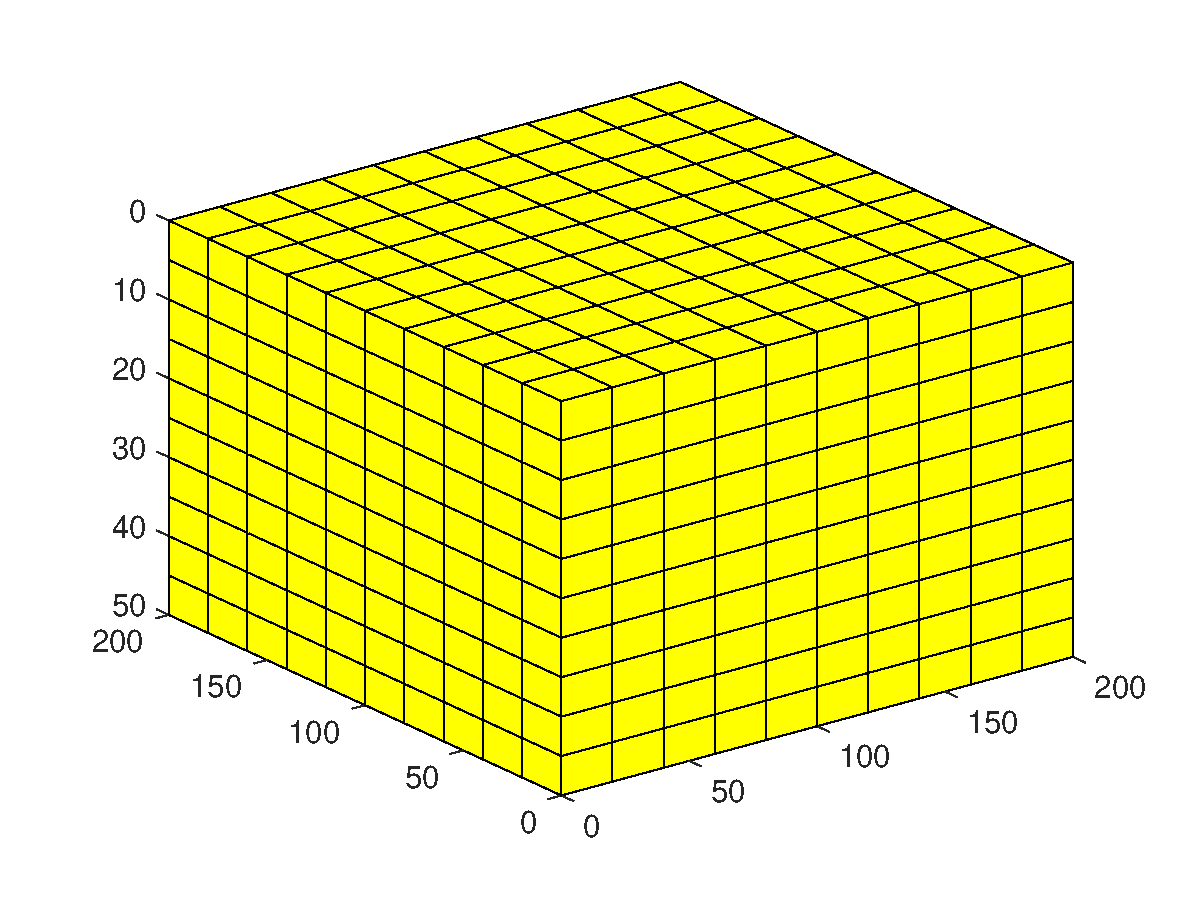
\includegraphics[width = \textwidth]{figures/flowSolver_grid.eps}
        \caption{Uniform $10\times 10 \times 10$ grid of the $200\times 200 \times 50 \text{m}^3$ big reservoir.}
        \label{fig:flowSolverGrid}
    \end{subfigure}
    \begin{subfigure}[t]{0.49\textwidth}
        \centering
        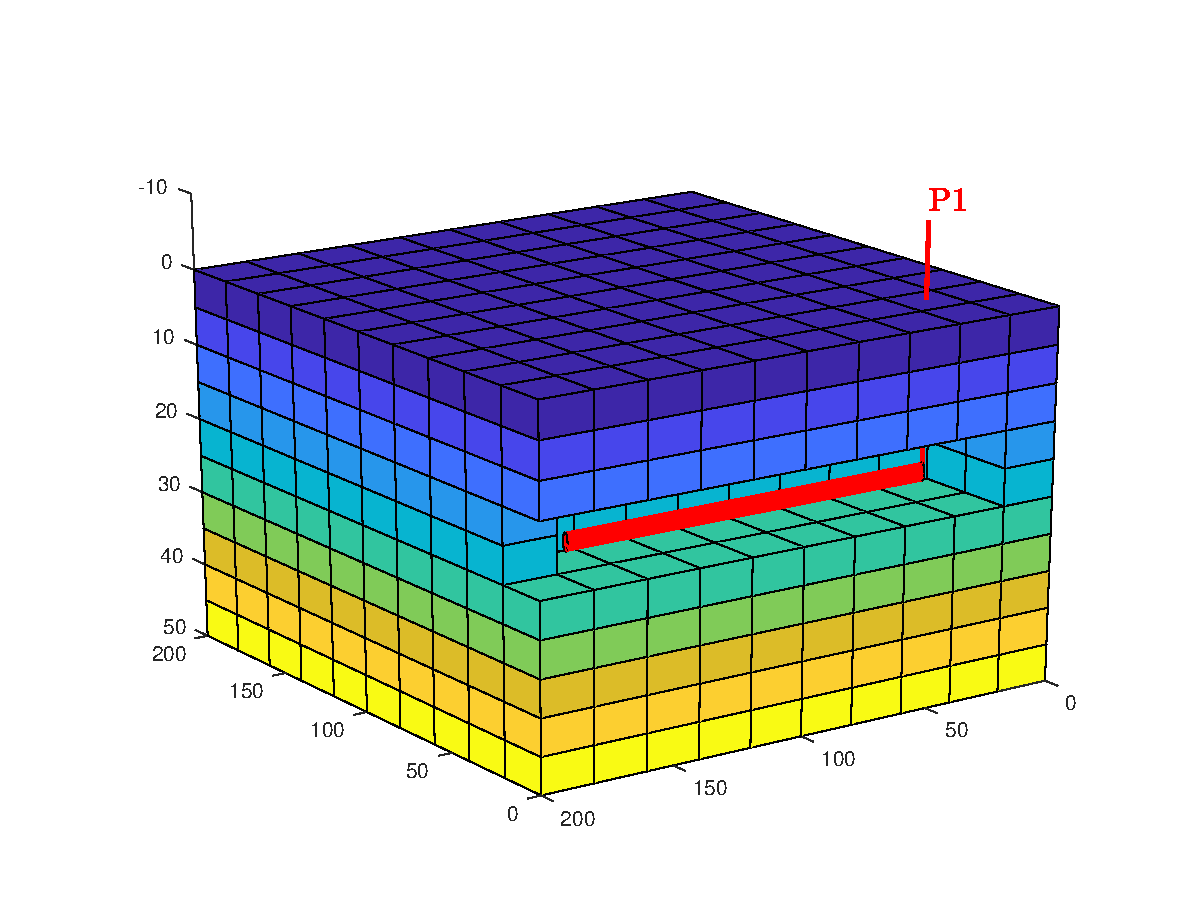
\includegraphics[width = \textwidth]{figures/flowSolver_gridWithWell.eps}
        \caption{Reservoir grid plotted with initial pressure and well P1. The well has replaced 8 grid elements. Some grid elements are removed to give a better visualization of the well.}
        \label{fig:flowSolverGridWithWell}
    \end{subfigure}
    \caption{}
\end{figure}
After initializing the grid we define the governing equations for the flow in the reservoir. We use a finite volume method to discretize in space and a backward Euler method to discretize in time. To solve the equations we use the Newton-Raphson method described in equation \eqref{eq:newtonRaphsonVector} with the residual form $\boldsymbol{F}(\boldsymbol{x}) = 0$. If we take a look at figure \ref{fig:flowSolverJacobian}, we can see the structure of the Jacobian of $F$. The first impression is that the matrix is very sparse. Except from a few nonzero points in row and column 1001 because of the well, the Jacobian consist of 7 diagonals (can look like 5 from perspective) with nonzero elements and the rest of the elements are 0. As we also can see from the figure there are only 6419 non-zero elements out of more than 1 million. It is clear that storing the whole $1002\times 1002$ matrix will be very inefficient. In MRST the Jacobians are stored as a list of sparse matrices where each Jacobian element in the list is the Jacobian with respect to one primary variable. 

\begin{figure}[htbp]
    \centering
    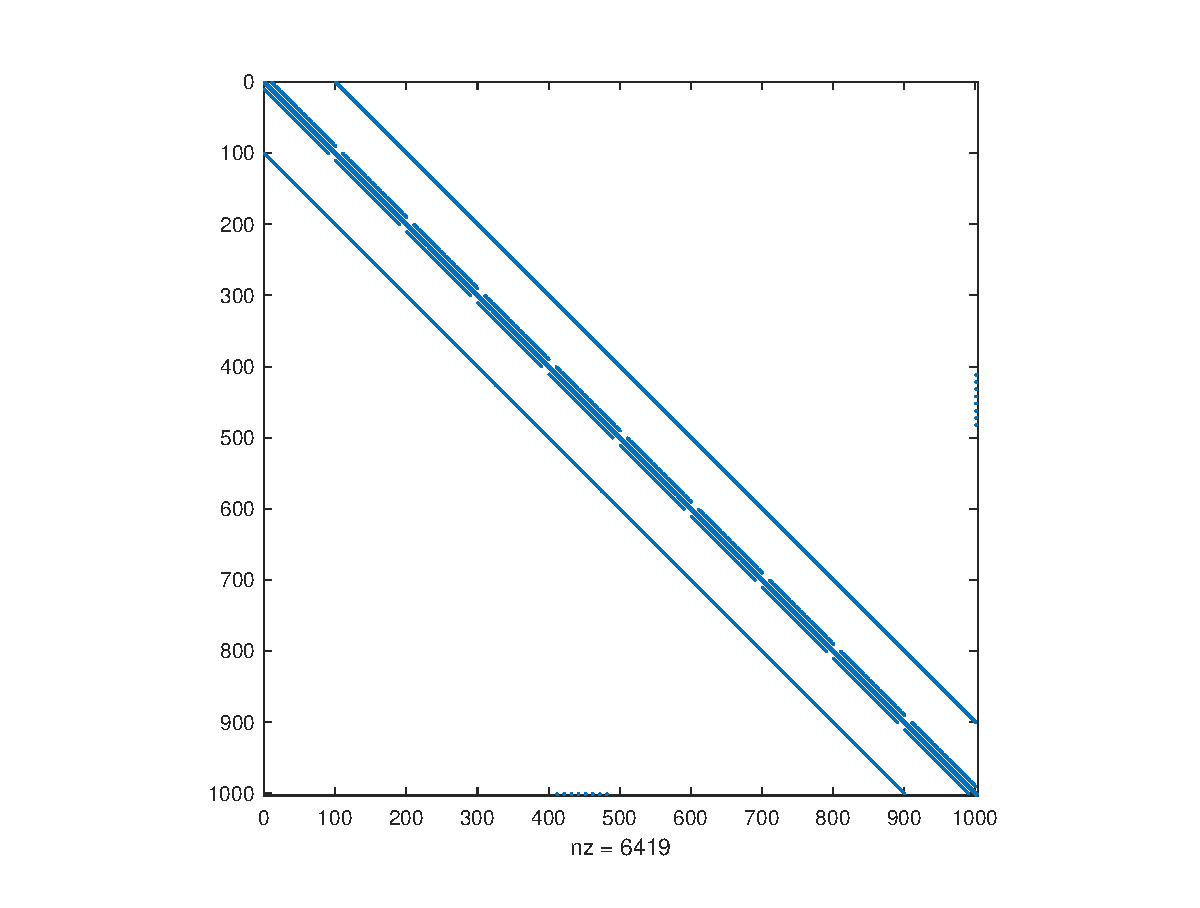
\includegraphics[width = 0.9\textwidth]{figures/flowSolver_Jacobian.eps}
    \caption{Structure of the $1002\times 1002$ Jacobian. There are 6419 non-zero elements.}
    \label{fig:flowSolverJacobian}
\end{figure}